\documentclass[11pt]{article}
\usepackage[T1]{fontenc}
\usepackage[utf8]{inputenc}
\usepackage{lmodern}
\usepackage[margin=0.9in]{geometry}
\usepackage{amsmath,amssymb,amsthm,mathtools}
\usepackage{microtype,booktabs,array,longtable,graphicx}
\usepackage{xcolor}
\usepackage{xurl}
\definecolor{ink}{HTML}{193C53}
\usepackage[colorlinks=true,linkcolor=ink,citecolor=ink,urlcolor=ink]{hyperref}
\hypersetup{pdftitle={Electrical laws for graph-coupled zeros},
pdfauthor={Research note prepared for Vladimir Reshetnikov},
pdfsubject={Exact transport formulas and a construction from Dirichlet GRH}}
\setcounter{tocdepth}{1}
\usepackage{enumitem}
\setlist{itemsep=3pt,topsep=5pt}
\usepackage{fancyhdr}
\pagestyle{fancy}
\fancyhf{}
\fancyhead[L]{\small Electrical laws for zeros}
\fancyhead[R]{\small 26 November 2026}
\fancyfoot[C]{\thepage}
\setlength{\headheight}{14pt}
\setlength{\emergencystretch}{2em}
\newtheorem{theorem}{Theorem}[section]
\newtheorem{lemma}[theorem]{Lemma}
\newtheorem{proposition}[theorem]{Proposition}
\newtheorem{corollary}[theorem]{Corollary}
\theoremstyle{definition}
\newtheorem{definition}[theorem]{Definition}
\theoremstyle{remark}
\newtheorem{remark}[theorem]{Remark}
\newcommand{\R}{\mathbb R}
\newcommand{\C}{\mathbb C}
\newcommand{\N}{\mathbb N}
\DeclareMathOperator{\ord}{ord}
\DeclareMathOperator{\diag}{diag}
\DeclareMathOperator{\nullity}{nullity}
\DeclareMathOperator{\tr}{tr}
\title{\textcolor{ink}{Electrical laws for graph-coupled zeros}\\[5pt]
\large Exact transport formulas and a construction from Dirichlet GRH}
\author{Research note prepared for Vladimir Reshetnikov}
\date{26 November 2026}

\begin{document}
\maketitle
\begin{abstract}
A connected weighted graph can combine a family of real-rooted polynomials
by a rooted-forest sum involving each polynomial and its first derivative.
We give an explicit symmetric matrix whose characteristic polynomial is
that sum.  The resulting zeros lie to the left, in ordered matching, of the
critical points of the product of the original polynomials.  Their exact
mean displacement is
\[
 \frac{1}{N(N-1)}\sum_{i<j}d_i d_jR_{ij},
\]
where $d_i$ are the input degrees, $N=\sum_i d_i$, and $R_{ij}$ are the
effective resistances of the graph.  Remarkably, the answer is independent
of all original zero locations.  Adding one edge gives a positive rank-one
matrix update and another exact displacement law.  We also prove a direct
entire-function version, with an exact formula for collisions and shared
zeros.  The cited Dirichlet GRH theorem supplies completed Dirichlet
$L$-functions to this construction, including complex characters after a
constant phase adjustment.  All proofs are included; rational-arithmetic
checks and reproducible figures accompany the paper.  The electrical
identities are the proposed new synthesis.  Their ingredients are classical,
and worldwide publication priority has not been established.
\end{abstract}
\vspace{5pt}
\noindent\textbf{Verification status.} Human-readable proofs and executed
exact finite checks.  The new theorems have not been formalized in Lean.
The upstream GRH development was inspected at a pinned revision; its full
build was not rerun for this note.
\tableofcontents
\clearpage
\section{Results, source analysis, and scope}\label{sec:context}

The main result is an exact relation between two objects: the zeros of a
polynomial constructed from a graph, and the electrical resistances of that
graph.  The relation can be computed before any of the input zero positions
are specified.  It also controls what happens when a single graph edge is
strengthened.  Theorem~\ref{thm:electrical} gives the full statement and
proof, and Theorem~\ref{thm:edge-law} gives the edge update.

The arithmetic application starts from the established Dirichlet
zero-location theorem in the supplied Lean repository.  A completed
$L$-function is rotated so that its critical line becomes the real axis.
The graph construction then gives further entire functions with all zeros
on that axis.  The finite electrical formulas apply to every finite packet
of zeros of the input functions.  The entire-function construction has its
own direct proof, so it does not require summing infinitely many zero
displacements.

\subsection{What the supplied sources actually establish}

The source inspection used the following fixed revisions:
\begin{center}
\small
\begin{tabular}{p{.26\textwidth}p{.66\textwidth}}
\toprule
Source & Revision or retrieval\\
\midrule
\texttt{lsernau/grh-lean} &
\path{72fead102f663d5c7a407964a13dc0cf9d977207}\\
\texttt{ProveIt} &
\path{4d7990202f9f106b2ffe8c209f073ad01d5e1987}\\
Wikipedia, Riemann hypothesis & Retrieved 26 November 2026; used for context\\
\bottomrule
\end{tabular}
\end{center}

The statement module of the compact Lean edition imports Mathlib and
formulates, among its endpoints, nonvanishing for every Dirichlet character
$\chi$ modulo every positive integer $q$:
\[
 \Re s>\tfrac12,\qquad (\chi\ne1\ \text{or}\ s\ne1)
 \quad\Longrightarrow\quad L(s,\chi)\ne0.
\]
It separately states the critical-strip zero-location theorem.  The
primitive-character version is a specialization, while the principal
character gives the zeta endpoint after the usual treatment of the pole.
The source does not state GRH for all Artin, Hecke, or automorphic
$L$-functions.\cite{grhsource}

The compact guide describes a comparison of covolumes obtained through
chains of theta lifts: sufficiently many short forms are compared with a
lower bound for integral forms.  This produces a one-sided estimate for a
smoothed prime remainder.  The final analytic step uses meromorphic
Laplace transforms, a quadratic twist that prevents residue cancellation,
and a Landau-type one-sign argument.  This is the mechanism visible in
the inspected guide and endgame modules.  The present graph argument is a
subsequent use of the zero-location endpoint and determinant methods; it
is not an alternative explanation of that theta-lift proof.\cite{grhguide}

The upstream README reports machine verification with the standard Lean
axioms \texttt{propext}, \texttt{Classical.choice}, and \texttt{Quot.sound},
and says the development has not been read through by a mathematician.
The Lean FRO and Mathlib Initiative's separate public statement endorses
Alp\"oge's original RH proof following statement comparison and independent
proof checks.  The retrieved Wikipedia article reports that development.
Those are externally reported checks; this packet makes no claim to have
reproduced the complete upstream build.\cite{grhsource,leanstatement,wikipedia}

\subsection{Comparison with ProveIt}

The organized GRH directory contains 61 research packets and explicitly
labels their placement as unreviewed.  At the pinned revision its local
\texttt{docs/incoming} directory also contains 39 later ZIP packets.  We
read all 61 organized delivery READMEs, extracted the text members of the
39 later archives, inspected their delivery summaries, and searched the
resulting corpus for the proposed construction.  This is a comparison of
the reported results and selected text, not an independent verification of
100 papers.  The exact inventory is recorded in the accompanying
provenance files.\cite{proveit}

Many plausible first directions are already represented there: Li
coefficients, Hankel and Ritz recovery of zeros, finite noisy certificates,
sampling, filtered prime races, torsion specialization, graph-tower
valuations, and symplectic or orthogonal matrix blocks.  The present
construction concerns a different graph operation: a rooted-forest sum of
functions and derivatives, an explicit symmetric compression, and an
electrical formula for the resulting zero displacement.  No matching
statement was found in the inspected corpus.

\subsection{What is classical and what is proposed as new}

The following ingredients are established mathematics: the matrix-forest
identity; compression formulas representing the critical points of a
polynomial; preservation of real zeros in the theory of stable
polynomials; matrix-valued Herglotz theory; and rank-one matrix inverse
identities.  Relevant primary sources include Chebotarev--Shamis,
Pereira, Borcea--Br\"and\'en, Reiffenstein, and
Simonov--Woracek.\cite{forests,pereira,bb,reiffenstein,simonov}

The contribution proposed here combines the rooted-forest derivative sum
with the explicit symmetric compression
\[
 K_G=(Q\Lambda Q-QVL^+V^{\mathsf T}Q)|_{\boldsymbol1_N^\perp}.
\]
From this we derive the exact resistance formula for zero transport,
its exact single-edge displacement law, and the completed
Dirichlet $L$-function specialization.  The proofs below establish the
claims as mathematical statements.  A targeted search did not locate this
precise electrical transport formula, but that is not a proof of first
publication.  In particular, the basic real-zero preservation theorem is
not presented as a newly discovered general principle.

The polynomial theorems are unconditional.  The arithmetic specialization
uses the supplied Dirichlet GRH result solely to put the completed
$L$-function zeros on the real axis.  It yields explicit differential
combinations; it does not identify new Euler products or prove a further
automorphic GRH.

% Standalone section: requires amsmath,amssymb,amsthm.
% The parent document should provide theorem, lemma, corollary, remark environments.
\section{An electrical transport theorem for real zeros}\label{sec:electrical}

Fix a connected undirected graph on $n\geq2$ labelled vertices, with positive
edge conductances.  Parallel edges may be combined by adding conductances.
Let $L$ be its weighted Laplacian, $L^+$ its Moore--Penrose inverse, and
\[
 \tau(G)=\sum_{T\text{ spanning tree}}\prod_{e\in T}w_e,
 \qquad
 R_{ij}=(e_i-e_j)^{\mathsf T}L^+(e_i-e_j).
\]
Thus $R_{ij}$ is the effective resistance between vertices $i$ and $j$.
At vertex $i$, place a monic real-rooted polynomial $p_i$ of degree
$d_i\geq1$, and put $N=d_1+\cdots+d_n$.
Repeated roots, including roots shared by different vertices, are allowed.

A rooted spanning forest consists of a spanning forest together with a
choice of one root in each of its tree components.  Write $\mathcal R(F)$
for its roots.  Define the following polynomial without any divisions:
\begin{equation}\label{eq:forest-polynomial}
 \mathcal P_G(z)=
 \sum_{F\text{ rooted spanning forest}}
 \left(\prod_{e\in F}w_e\right)
 \left(\prod_{i\in\mathcal R(F)}p_i'(z)\right)
 \left(\prod_{i\notin\mathcal R(F)}p_i(z)\right).
\end{equation}
The empty edge set is included, and contributes $\prod_i p_i'$.
The constructions below show that $\mathcal P_G$ is never the zero
polynomial and has degree $N-1$.

List the roots of the input polynomials, with multiplicity and in vertex
blocks, as $r_1,\ldots,r_N$.  Set
\[
 \Lambda=\operatorname{diag}(r_1,\ldots,r_N),\qquad
 V_{ai}=\begin{cases}1&\text{root }a\text{ belongs to }p_i,\\0&\text{otherwise},\end{cases}
 \qquad Q=I_N-\frac{\boldsymbol 1_N\boldsymbol 1_N^{\mathsf T}}{N}.
\]
Here $V$ has $N$ rows and $n$ columns.  Let
$H=\boldsymbol 1_N^\perp$ and use restriction to $H$ whenever a determinant
or eigenvalue of a compressed matrix is taken.  Define
\[
 A_\infty=(Q\Lambda Q)|_H,\qquad
 B_G=(QV L^+V^{\mathsf T}Q)|_H,\qquad K_G=A_\infty-B_G.
\]

\begin{theorem}[Exact compression and electrical transport]\label{thm:electrical}
The following identity holds for every complex $z$:
\begin{equation}\label{eq:compression-identity}
 \boxed{\quad\mathcal P_G(z)=N\tau(G)\det_H(zI_H-K_G).\quad}
\end{equation}
In particular $\mathcal P_G$ has exactly $N-1$ real zeros, with multiplicity.
Let these zeros be $\lambda_1\leq\cdots\leq\lambda_{N-1}$, and let
$\beta_1\leq\cdots\leq\beta_{N-1}$ be the zeros of
$(\prod_i p_i)'$.  Then
\begin{equation}\label{eq:root-upper-bound}
 0\leq\beta_k-\lambda_k\leq\|B_G\|\qquad(1\leq k\leq N-1),
\end{equation}
and
\begin{equation}\label{eq:resistance-sum}
 \boxed{\quad
 \sum_{k=1}^{N-1}(\beta_k-\lambda_k)
 =\frac1N\sum_{i<j}d_i d_jR_{ij}.
 \quad}
\end{equation}
Consequently the empirical probability measures
\[
 \mu_G=\frac1{N-1}\sum_k\delta_{\lambda_k},\qquad
 \nu=\frac1{N-1}\sum_k\delta_{\beta_k}
\]
satisfy the exact optimal-transport formula
\begin{equation}\label{eq:wasserstein-exact}
 \boxed{\quad W_1(\mu_G,\nu)
 =\frac{\sum_{i<j}d_i d_jR_{ij}}{N(N-1)}.\quad}
\end{equation}
Here $W_1$ denotes the minimum average distance needed to transport one
probability measure into the other.  The value in
\eqref{eq:wasserstein-exact} is independent of every input root location.
The bound $W_\infty(\mu_G,\nu)\leq\|B_G\|$ is sharp over the permitted
input polynomials, even with the graph and the degrees fixed.
\end{theorem}

\begin{proof}
We first establish the elementary forest determinant identity
\begin{equation}\label{eq:forest-det}
 \det(L+\operatorname{diag}(x_1,\ldots,x_n))
 =\sum_{F\text{ rooted spanning forest}}
   \left(\prod_{e\in F}w_e\right)\prod_{i\in\mathcal R(F)}x_i.
\end{equation}
One proof adds a new vertex $0$ and an edge of weight $x_i$ from $0$ to
each vertex $i$.  The matrix-tree theorem identifies the left side with
the spanning-tree polynomial of the enlarged graph.  Removing $0$ from
such a tree leaves a spanning forest; each component has exactly one
vertex formerly adjacent to $0$, which becomes its root.  This is a
weight-preserving bijection.  Since it proves a polynomial identity, no
sign assumption on the variables $x_i$ is required.

Away from the input roots, substitute $x_i=p_i'/p_i$ in
\eqref{eq:forest-det} and multiply by $p=\prod_i p_i$.  This gives
\begin{equation}\label{eq:meromorphic-determinant}
 \mathcal P_G(z)=p(z)
 \det\left(L+\operatorname{diag}\left(\frac{p_i'(z)}{p_i(z)}\right)\right).
\end{equation}
By the definition of $V$ and $\Lambda$,
\[
 V^{\mathsf T}(zI_N-\Lambda)^{-1}V
  =\operatorname{diag}\left(\frac{p_i'(z)}{p_i(z)}\right).
\]
The Schur complement of the upper-left block therefore yields the
polynomial identity
\begin{equation}\label{eq:bordered-determinant}
 \mathcal P_G(z)=
 \det\begin{pmatrix}zI_N-\Lambda&V\\-V^{\mathsf T}&L\end{pmatrix}.
\end{equation}
It suffices to establish this first for $z$ outside the finite input
zero set, because both sides are polynomials.

Choose an orthonormal basis of $\mathbb R^n$ starting with
$u=\boldsymbol1_n/\sqrt n$ and otherwise consisting of Laplacian
eigenvectors.  Eliminate the positive-eigenvalue block of $L$ in
\eqref{eq:bordered-determinant}.  The result is
\[
 \det{}'(L)
 \det\begin{pmatrix}
 zI_N-\Lambda+VL^+V^{\mathsf T}&Vu\\
 -u^{\mathsf T}V^{\mathsf T}&0
 \end{pmatrix},
\]
where $\det{}'(L)$ is the product of the $n-1$ positive eigenvalues.
The identity $Vu=\boldsymbol1_N/\sqrt n$ gives
$\|Vu\|^2=N/n$ and $(Vu)^\perp=H$.
For any $N\times N$ matrix $C$ and any nonzero real vector $b$,
\[
 \det\begin{pmatrix}C&b\\-b^{\mathsf T}&0\end{pmatrix}
   =\|b\|^2\det_{b^\perp}(P_{b^\perp}C|_{b^\perp}).
\]
Indeed, in a basis ending with $b/\|b\|$, expansion along the last row
and then the last column gives this equality, including its positive
sign.  Finally $\det{}'(L)=n\tau(G)$ by the matrix-tree theorem.
Together these facts prove \eqref{eq:compression-identity}.

The matrix $K_G$ is real symmetric.  Also $B_G\succeq0$ because
$L^+\succeq0$.  The usual compression identity for derivatives gives
\begin{equation}\label{eq:differentiator}
 \det_H(zI_H-A_\infty)=\frac1N p'(z).
\end{equation}
For completeness, if $e=\boldsymbol1_N/\sqrt N$, the cofactor formula
for a compression says that the left side is
$p(z)e^{\mathsf T}(zI_N-\Lambda)^{-1}e$ whenever the inverse exists.
This is $p(z)N^{-1}\sum_a(z-r_a)^{-1}=p'(z)/N$; polynomial
continuation proves the identity everywhere.  The min--max principle
applied to
$A_\infty-\|B_G\|I_H\preceq K_G\preceq A_\infty$
now proves \eqref{eq:root-upper-bound}.

Put $d=(d_1,\ldots,d_n)^{\mathsf T}$ and
$D=\operatorname{diag}(d_1,\ldots,d_n)$.  Since
$V^{\mathsf T}V=D$ and $V^{\mathsf T}\boldsymbol1_N=d$,
\begin{align*}
 \sum_k(\beta_k-\lambda_k)
 &=\operatorname{tr}B_G
 =\operatorname{tr}\left[L^+\left(D-\frac{dd^{\mathsf T}}N\right)\right]\\
 &=\sum_i d_i(L^+)_{ii}-\frac1N d^{\mathsf T}L^+d
 =\frac1N\sum_{i<j}d_i d_jR_{ij}.
\end{align*}
The last equality follows by expanding
$R_{ij}=(L^+)_{ii}+(L^+)_{jj}-2(L^+)_{ij}$.
For equal-weight measures on the line, an optimal coupling matches
the atoms in increasing order.  Alternatively, the ordered matching
attains the difference of the means here because
$\lambda_k\leq\beta_k$, and every coupling has average distance at
least the absolute difference of the means.  This proves
\eqref{eq:wasserstein-exact} directly.

The ordered matching also proves the $W_\infty$ bound.  To prove
sharpness choose $p_i(z)=(z-c)^{d_i}$ for a common real $c$.
Then $A_\infty=cI_H$; hence the largest displacement is exactly
the largest eigenvalue of $B_G$, namely $\|B_G\|$.
\end{proof}

\begin{corollary}[Electrical barycentre law]\label{cor:barycentre}
The mean of the $N-1$ graph zeros is
\begin{equation}\label{eq:barycentre}
 \frac1{N-1}\sum_k\lambda_k
  =\frac1N\sum_{a=1}^N r_a
   -\frac{\sum_{i<j}d_i d_jR_{ij}}{N(N-1)}.
\end{equation}
\end{corollary}
\begin{proof}
The trace of $A_\infty$ is
$\operatorname{tr}\Lambda-N^{-1}\boldsymbol1_N^{\mathsf T}\Lambda\boldsymbol1_N
=(N-1)N^{-1}\sum_a r_a$.  Substitute this in
\eqref{eq:resistance-sum}.
\end{proof}

\section{Adding one edge: exact root motion}\label{sec:edge-motion}

An edge may be strengthened or inserted.  Fix distinct vertices $a,b$,
put $b_e=e_a-e_b$, and let $L_h=L+h b_e b_e^{\mathsf T}$ for $h\geq0$.
Define quantities using the original connected graph:
\[
 R_e=b_e^{\mathsf T}L^+b_e>0,\qquad
 q_e=QV L^+b_e\in H,\qquad
 \alpha(h)=\frac{h}{1+hR_e}.
\]

\begin{theorem}[Exact edge law]\label{thm:edge-law}
The associated symmetric matrices satisfy
\begin{equation}\label{eq:rank-one-edge}
 \boxed{\quad K_{G_h}=K_G+\frac{h}{1+hR_e}q_e q_e^{\mathsf T}.\quad}
\end{equation}
In particular the ordered graph zeros obey
\[
 \lambda_k(G)\leq\lambda_k(G_h)\leq\lambda_{k+1}(G)
 \quad(1\leq k<N-1),\qquad
 \lambda_{N-1}(G)\leq\lambda_{N-1}(G_h).
\]
Their total displacement is exactly
\begin{equation}\label{eq:edge-total-displacement}
 \boxed{\quad
 \sum_{k=1}^{N-1}\bigl(\lambda_k(G_h)-\lambda_k(G)\bigr)
 =\frac{h}{1+hR_e}\|q_e\|^2.
 \quad}
\end{equation}
This is strictly positive for $h>0$ and does not depend on the input
root locations.  Equivalently,
\[
 W_1(\mu_G,\mu_{G_h})
 =\frac{h\,\|q_e\|^2}{(N-1)(1+hR_e)}.
\]
At a simple eigenvalue, for a normalized real eigenvector $u_k(h)$,
\begin{equation}\label{eq:edge-velocity}
 \frac{d\lambda_k(G_h)}{dh}
 =\frac{|u_k(h)^{\mathsf T}q_e|^2}{(1+hR_e)^2}.
\end{equation}
The total displacement is bounded above by $\|q_e\|^2/R_e$ and
approaches this value as the new conductance tends to infinity.
\end{theorem}

\begin{proof}
On $\boldsymbol1_n^\perp$, the matrix $L$ is positive definite.  The
rank-one inverse identity on that subspace gives
\[
 L_h^+=L^+-\frac{h}{1+hR_e}
                 L^+b_e b_e^{\mathsf T}L^+.
\]
Both sides vanish on $\boldsymbol1_n$, so this is also an identity
on $\mathbb R^n$.  Substitution in the definition of $K_G$ proves
\eqref{eq:rank-one-edge}.  Eigenvalue monotonicity and rank-one
interlacing give the displayed inequalities.  Taking traces proves
\eqref{eq:edge-total-displacement}, and ordered matching proves the
$W_1$ formula.

To check strict positivity, suppose $QV L^+b_e=0$ and write
$x=L^+b_e\in\boldsymbol1_n^\perp$.  Then $Vx$ is constant on all
$N$ coordinates.  As every vertex block is nonempty, all coordinates
of $x$ are equal.  Hence $x=0$, contradicting $Lx=b_e\ne0$.
Thus $q_e\ne0$.  Finally, differentiating the rank-one matrix
identity at a simple eigenvalue yields
\eqref{eq:edge-velocity}, since $\alpha'(h)=(1+hR_e)^{-2}$.
\end{proof}

\begin{remark}[Everything in the displacement budget is electrical]
The vector $q_e$ need not be formed in the $N$-dimensional root space:
\[
 \|q_e\|^2=b_e^{\mathsf T}L^+
      \left(D-\frac{dd^{\mathsf T}}N\right)L^+b_e.
\]
Thus the budget is determined by the graph, the chosen edge, and the
input degrees.  Eigenvectors and the actual zero locations determine
how that fixed budget is distributed among individual zeros.
\end{remark}

\section{A monotone bridge between two derivative constructions}

Scale every conductance by $t>0$ and write $\lambda_k(t)$ for the
zeros of the resulting graph polynomial.  Since $(tL)^+=t^{-1}L^+$,
\begin{equation}\label{eq:uniform-scale}
 K_t=A_\infty-t^{-1}B_G.
\end{equation}
All $N-1$ ordered zeros are nondecreasing with $t$, and they tend to the zeros
of $(\prod_i p_i)'$ as $t\to\infty$.  More precisely,
\[
 0\leq\beta_k-\lambda_k(t)\leq\frac{\|B_G\|}{t},\qquad
 W_1(\mu_{tG},\nu)=
 \frac{\sum_{i<j}d_i d_jR_{ij}}{tN(N-1)}.
\]
There is also a precise small-coupling limit.

\begin{corollary}[Small-coupling limit]\label{cor:small-coupling}
Exactly $n-1$ graph zeros tend to $-\infty$ as $t\downarrow0$.
The other $N-n$ zeros tend, with multiplicity and in increasing order,
to the zeros of $\prod_i p_i'$.  When $N=n$, this latter list is empty.
\end{corollary}
\begin{proof}
On $H$, the matrix $B_G$ has kernel $\ker V^{\mathsf T}$.
Indeed $v^{\mathsf T}B_Gv=0$ is equivalent to
$V^{\mathsf T}v\in\operatorname{span}(\boldsymbol1_n)$; because
$v\perp\boldsymbol1_N$, the sum of the coordinates of
$V^{\mathsf T}v$ is zero, so the latter vector must vanish.
The map $V$ has rank $n$, and hence $B_G$ has rank $n-1$ on $H$.
In the orthogonal decomposition
$H=\operatorname{ran}B_G\oplus\ker B_G$, write
\[
 K_t=\begin{pmatrix}A_{11}-t^{-1}B_1&A_{12}\\
 A_{21}&A_{22}\end{pmatrix},\qquad B_1\succ0.
\]
The first $n-1$ eigenvalues tend to $-\infty$ by min--max.
For $z$ in any fixed bounded set, the inverse of
$zI-A_{11}+t^{-1}B_1$ is $O(t)$, uniformly as $t\downarrow0$.
The complementary Schur determinant therefore tends to
$\det(zI-A_{22})$.  Thus the remaining $N-n$ eigenvalues tend to
the eigenvalues of $A_{22}$, including multiplicity.  This also follows
by applying polynomial continuity to the Schur determinant and using
interlacing to keep these eigenvalues bounded.

Finally $\ker V^{\mathsf T}$ is the direct sum, over the vertex blocks,
of the subspaces whose coordinates sum to zero.  The compression of
$\Lambda$ to these subspaces has characteristic polynomial
$\prod_i(p_i'/d_i)$ by \eqref{eq:differentiator} applied separately
to each block.  These are exactly the asserted finite limiting zeros.
\end{proof}

\section{An exact three-vertex example}\label{sec:exact-example}

Put $p_1(z)=z+1$, $p_2(z)=z$, and $p_3(z)=z-1$ on a three-vertex
path, with each of its two edges having conductance $t>0$.  Enumerating
the rooted forests gives
\[
 \mathcal P_t(z)=1+4tz+t^2(3z^2-1),\qquad
 \lambda_\pm(t)=\frac{-2\pm\sqrt{1+3t^2}}{3t}.
\]
Both zeros increase to $\pm1/\sqrt3$, the zeros of
$(z^3-z)'$.  The three pairwise effective resistances are
$1/t,1/t,2/t$.  The exact transport distance is therefore
\[
 W_1(\mu_t,\nu)=\frac{2}{3t}.
\]
At $t=1$, the graph polynomial is $z(3z+4)$, whose zeros are
$-4/3$ and $0$.  Thus the real-zero theorem does not assert containment
in the interval of the original roots: one new zero lies to the left
of all three input roots.  What is controlled exactly is its ordered
displacement from the zeros of the derivative of their product.

\paragraph{Scope.}
All trace, barycentre and transport formulas in this section concern
finite polynomials.  Applying a formally infinite sum to completed
$L$-functions would require a separate convergence or renormalization
theorem.  The entire-function real-zero and local collision results
do not require such a sum and can be proved directly from logarithmic
derivatives.

\begin{figure}[tbp]
 \centering
 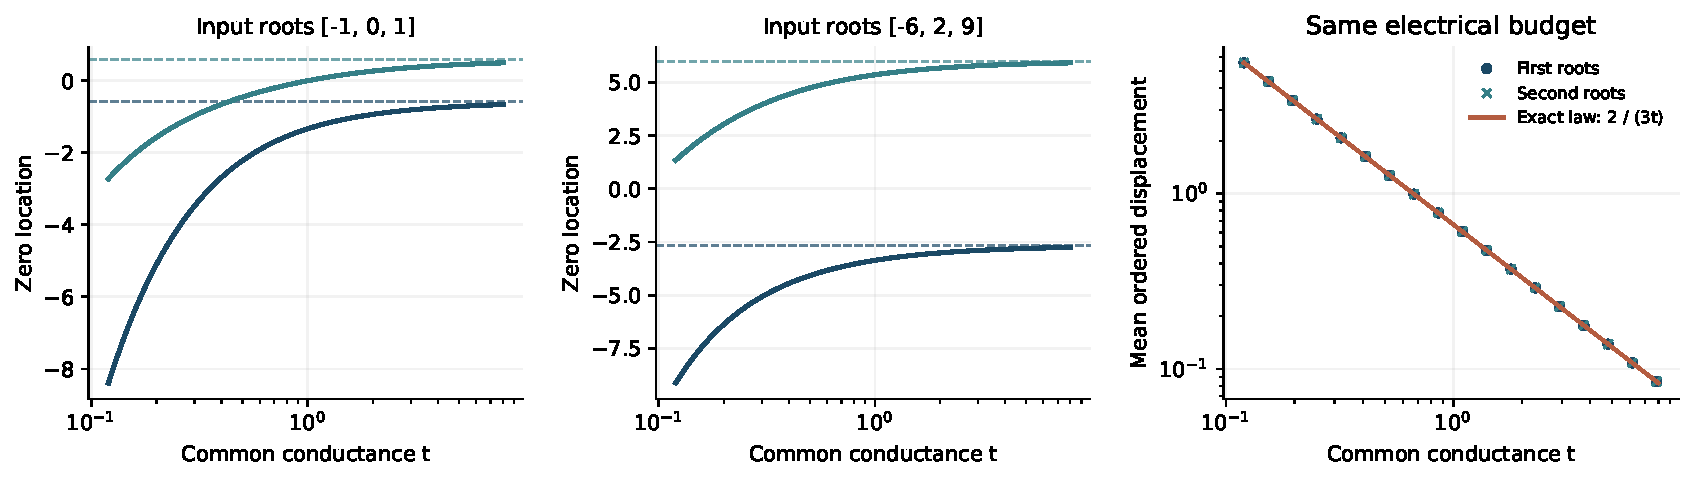
\includegraphics[width=\textwidth]{figures/electrical_transport.pdf}
 \caption{Two different sets of input zeros on the same three-vertex path.
 Solid curves are the graph zeros as the common conductance increases;
 dashed lines are the critical points of the product.  Both examples have
 the same exact mean displacement $2/(3t)$.  The plot is numerical; the
 identity is proved in Theorem~\ref{thm:electrical}.}
 \label{fig:transport}
\end{figure}
% Requires amsmath,amssymb,amsthm; theorem,lemma,corollary,remark environments.
% Bibliography keys used: reiffenstein, dlmfdirichlet.
\section{Entire functions, collisions, and zero counting}
\label{sec:entire-graph}

The finite compression theorem has an entire-function counterpart.
Its real-zero mechanism is the classical sign of a logarithmic derivative
of a real canonical product.  In matrix language this is a special case
of meromorphic Herglotz theory and its higher-order interlacing;
we do not claim that mechanism as new.\cite{reiffenstein}
We give direct proofs to make the multiplicities and all pole cancellations
in the present construction explicit.

\subsection{The precise analytic class}

Let $F_1,\ldots,F_n$ be nonzero entire functions with representations
\begin{equation}\label{eq:real-canonical-product}
 F_i(z)=c_i z^{m_i}e^{b_i z}
 \prod_{\rho\in\mathcal Z_i}
 \left(1-\frac z\rho\right)e^{z/\rho},
 \qquad
 c_i\in\mathbb R\setminus\{0\},\quad b_i\in\mathbb R,\quad m_i\geq0.
\end{equation}
Here $\mathcal Z_i$ is a possibly empty multiset of nonzero real numbers,
each zero is listed with multiplicity,
$\sum_{\rho\in\mathcal Z_i}|\rho|^{-2}<\infty$, and the product converges
locally uniformly.  Assume that each $F_i$ has at least one zero:
$m_i+|\mathcal Z_i|>0$.
These hypotheses hold, in particular, for real entire functions of order
at most one with at least one zero and with all zeros real, by Hadamard
factorization.  They also include the polynomial inputs above.
No assumption that $F_i(0)\neq0$ is made.

Write $g_i=F_i'/F_i$ away from the zeros of $F_i$.
Termwise logarithmic differentiation of
\eqref{eq:real-canonical-product} gives
\begin{equation}\label{eq:logder-canonical}
 g_i(z)=b_i+\frac{m_i}{z}
   +\sum_{\rho\in\mathcal Z_i}
       \left(\frac1{z-\rho}+\frac1\rho\right).
\end{equation}
The sum and its derivative converge uniformly on compact sets avoiding
the zeros: for large $|\rho|$ the summand in \eqref{eq:logder-canonical}
is $O(|\rho|^{-2})$, uniformly on each such compact set.

\begin{lemma}[Strict half-plane sign]\label{lem:strict-logder}
For $z=x+iy$ with $y\neq0$,
\begin{equation}\label{eq:logder-imaginary}
 \operatorname{Im}g_i(z)
 =-y\left(\frac{m_i}{|z|^2}
       +\sum_{\rho\in\mathcal Z_i}\frac1{|z-\rho|^2}\right).
\end{equation}
At real $x$ with $F_i(x)\neq0$,
\begin{equation}\label{eq:logder-decrease}
 -g_i'(x)=
 \frac{m_i}{x^2}
       +\sum_{\rho\in\mathcal Z_i}\frac1{(x-\rho)^2}>0.
\end{equation}
Terms involving $m_i$ are omitted when $m_i=0$.
\end{lemma}
\begin{proof}
The constants $b_i$ and $1/\rho$ are real, and
$\operatorname{Im}(z-\rho)^{-1}=-y/|z-\rho|^2$.
This proves \eqref{eq:logder-imaginary}.
Differentiating \eqref{eq:logder-canonical} gives
\eqref{eq:logder-decrease}.
At least one nonnegative term in each parenthesized sum is positive,
because $F_i$ has at least one zero.
\end{proof}

The analytic class matters.  Real zero location alone, without a growth
or canonical-product restriction, is insufficient: $F(z)=ze^{z^2}$ has
only a real zero, whereas $F'(z)=e^{z^2}(1+2z^2)$ has nonreal zeros.
Likewise a zero-free exponential has constant logarithmic derivative
and does not satisfy the strict inequality needed below.

\subsection{A determinant without division}

Let $A$ be an $n$-by-$n$ Hermitian matrix, constant in $z$.  For a subset
$S\subseteq[n]=\{1,\ldots,n\}$, write $A[S]$ for the corresponding
principal submatrix, with $\det A[\varnothing]=1$.  Define
\begin{align}
 \mathcal P_A(z)
 &=\det\!\left(
       \operatorname{diag}(F_1(z),\ldots,F_n(z))A+
       \operatorname{diag}(F'_1(z),\ldots,F'_n(z))
          \right) \label{eq:entire-determinant}\\
 &=\sum_{S\subseteq[n]}
       \det A[S^{\mathrm c}]
       \prod_{i\in S}F_i'(z)
       \prod_{j\notin S}F_j(z). \label{eq:principal-minor-entire}
\end{align}
The second equality follows by multilinearity in the rows of the
determinant.  It proves directly that $\mathcal P_A$ is entire.
Every principal minor of a Hermitian matrix is real, so $\mathcal P_A$
is a real entire function.
Away from the input zeros, put
\[
 M_A(z)=A+\operatorname{diag}(g_1(z),\ldots,g_n(z)).
\]
Then
\begin{equation}\label{eq:entire-meromorphic-factorization}
 \mathcal P_A(z)=\left(\prod_iF_i(z)\right)\det M_A(z).
\end{equation}

\begin{theorem}[Real zeros under Hermitian coupling]\label{thm:entire-real-zeros}
The entire function $\mathcal P_A$ is not identically zero and all of
its zeros are real.
For $A=L$, a weighted graph Laplacian, it is precisely the rooted-forest
expression \eqref{eq:forest-polynomial} with $p_i$ replaced by $F_i$.
\end{theorem}
\begin{proof}
Take $z$ in the upper half-plane.  All $F_i(z)$ are nonzero.
If $M_A(z)v=0$ for a nonzero vector $v$, Hermiticity of $A$ and
Lemma~\ref{lem:strict-logder} give
\[
 0=\operatorname{Im}\bigl(v^*M_A(z)v\bigr)
   =\sum_i|v_i|^2\operatorname{Im}g_i(z)<0,
\]
a contradiction.  Thus \eqref{eq:entire-meromorphic-factorization}
is nonzero throughout the upper half-plane.  Since $\mathcal P_A$ is
real entire, it is nonzero throughout the lower half-plane as well.
The forest assertion follows from the polynomial identity
\eqref{eq:forest-det}; its substitution is first valid off the input
zeros, and the entire expressions then agree everywhere.
\end{proof}

\subsection{An exact formula at collisions}

A product formula written with logarithmic derivatives can conceal
cancellation at a shared zero.  The following formula resolves every
such collision, including multiple and central zeros.

Fix $\lambda\in\mathbb R$, and define
\[
 I=\{i:F_i(\lambda)=0\},\qquad J=[n]\setminus I,\qquad
 \mu_i=\operatorname{ord}_{\lambda}F_i\quad(i\in I).
\]
Define the complementary Hermitian matrix
\begin{equation}\label{eq:collision-complement}
 C_\lambda=A[J]+\operatorname{diag}(g_j(\lambda):j\in J),
 \qquad k_\lambda=\dim\ker C_\lambda.
\end{equation}
If $J$ is empty, its nullity is defined to be zero.

\begin{theorem}[Exact collision order]\label{thm:collision-order}
For every real $\lambda$,
\begin{equation}\label{eq:collision-order}
 \boxed{\quad
 \operatorname{ord}_{\lambda}\mathcal P_A
    =\sum_{i\in I}(\mu_i-1)+k_\lambda .
 \quad}
\end{equation}
When $I$ is empty, this says that the multiplicity of a zero away from
the input zeros equals the nullity of $M_A(\lambda)$.
\end{theorem}
\begin{proof}
Set $t=z-\lambda$.  For $i\in I$ write
$F_i(\lambda+t)=t^{\mu_i}h_i(t)$ with $h_i(0)\neq0$.
The $I$-by-$I$ block of $M_A(\lambda+t)$ is
\[
 B(t)=t^{-1}D+E(t),\qquad
 D=\operatorname{diag}(\mu_i:i\in I),
\]
where $E$ is analytic near zero.  Hence
\[
 B(t)^{-1}=tD^{-1}+O(t^2),\qquad
 \det B(t)=t^{-|I|}\det D\,(1+O(t)).
\]
The Schur complement of this block is analytic near zero:
\begin{align*}
 S(t)&=A[J]+\operatorname{diag}(g_j(\lambda+t):j\in J)
                   -A[J,I]B(t)^{-1}A[I,J]\\
     &=C_\lambda+tD_\lambda+O(t^2),
\end{align*}
where
\begin{equation}\label{eq:collision-negative-derivative}
 D_\lambda=
   \operatorname{diag}(g_j'(\lambda):j\in J)
        -A[J,I]D^{-1}A[I,J]\prec0
\end{equation}
when $J$ is nonempty.  Indeed the first term is strictly negative
definite by \eqref{eq:logder-decrease}, and the term subtracted from it
is positive semidefinite.

We verify explicitly that $\det S(t)$ has order $k_\lambda$.
Use the orthogonal decomposition
$\mathbb C^J=\ker C_\lambda\oplus(\ker C_\lambda)^\perp$.
On the second summand $C_\lambda$ is invertible.  Taking its Schur
complement reduces the first block to
\[
 t\,D_\lambda|_{\ker C_\lambda}+O(t^2).
\]
Cross-block contributions start in order $t^2$, since the off-diagonal
blocks of $C_\lambda$ in this decomposition vanish.
The compression of $D_\lambda$ to the kernel is negative definite,
so its determinant is nonzero.  Thus
$\operatorname{ord}_0\det S=k_\lambda$.
This argument also covers a zero-dimensional kernel; the empty
determinant is one.

Finally, the factors $\prod_{i\in I}F_i$ supply order
$\sum_{i\in I}\mu_i$, $\det B(t)$ removes $|I|$, and all $F_j(\lambda)$
for $j\in J$ are nonzero.  Equation
\eqref{eq:entire-meromorphic-factorization} now gives
\eqref{eq:collision-order}.
If $I$ is empty, apply the kernel-compression argument directly to
$M_A(\lambda+t)$, whose derivative is strictly negative definite.
If $J$ is empty, the first block alone gives the asserted order.
\end{proof}

No simplicity or noncoincidence assumption is hidden in this formula.
For example, if every input has a simple zero at $\lambda$, then
$I=[n]$, $J=\varnothing$, and $\mathcal P_A(\lambda)\neq0$:
the apparent common zero is removed completely.

\subsection{A bounded discrepancy on every interval}

Let $n_+(B)$ denote the number of strictly positive eigenvalues of a
Hermitian matrix $B$, counted with multiplicity.  For a nonzero entire
function $F$, let $N_F(a,b)$ count its real zeros in $(a,b)$ with
multiplicity.

\begin{theorem}[Exact zero-count identity]\label{thm:entire-count}
Let $a<b$ be real, and suppose neither endpoint is a zero of any $F_i$
or of $\mathcal P_A$.  Then
\begin{equation}\label{eq:inertia-count}
 \boxed{\quad
 N_{\mathcal P_A}(a,b)
  =\sum_iN_{F_i}(a,b)
     +n_+(M_A(a))-n_+(M_A(b)).
 \quad}
\end{equation}
In particular,
\begin{equation}\label{eq:count-discrepancy}
 \left|N_{\mathcal P_A}(a,b)-\sum_iN_{F_i}(a,b)\right|\leq n.
\end{equation}
If the interval contains no input zero, it contains at most $n$ zeros
of $\mathcal P_A$, counted with multiplicity.
\end{theorem}
\begin{proof}
On any interval without input zeros,
\[
 M_A'(x)=\operatorname{diag}(g_i'(x))\prec0.
\]
At a zero of $\det M_A$ with kernel dimension $k$, the same compression
argument used above shows that the $k$ zero eigenvalues cross from
positive to negative as $x$ increases.  Its positive inertia therefore
drops by $k$, which is exactly the multiplicity of $\mathcal P_A$ there.

Now cross an input zero $\lambda$ with notation as in
Theorem~\ref{thm:collision-order}.  For small negative $t$, the block
$B(t)$ has $|I|$ negative eigenvalues; for small positive $t$, it has
$|I|$ positive eigenvalues.  Hermitian block elimination preserves
inertia, so the remaining eigenvalues are counted by $S(t)$.
Its $k_\lambda$ zero eigenvalues cross from positive to negative by
\eqref{eq:collision-negative-derivative}; its other eigenvalues retain
their signs.  Consequently
\[
 n_+(M_A(\lambda+0))-n_+(M_A(\lambda-0))
       =|I|-k_\lambda
       =\sum_{i\in I}\mu_i
          -\operatorname{ord}_{\lambda}\mathcal P_A.
\]
There are only finitely many zeros of these nonzero entire functions
in a compact interval.  Summing these jumps, including the ordinary
zeros between poles, telescopes to \eqref{eq:inertia-count}.
Since positive inertia lies between zero and $n$, the two remaining
claims follow.
\end{proof}

The discrepancy bound is sharp even for connected graph Laplacians.
Take $F_i(z)=z$ for every $i$.  If the nonzero eigenvalues of $L$ are
$\ell_2,\ldots,\ell_n>0$, then
\[
 \mathcal P_L(z)=\prod_{j=2}^n(1+\ell_jz).
\]
An interval sufficiently close to zero contains all $n$ input zeros
and no output zero, attaining discrepancy $-n$.

\subsection{Local motion under a positive coupling change}

A local monotonicity statement survives for entire inputs, although
the finite resistance sum in \eqref{eq:resistance-sum} is not an
unregularized sum over infinitely many zeros.

\begin{corollary}[Velocity of a simple zero]\label{cor:entire-velocity}
Let $A(t)=A_0+tB$ with $B\succeq0$ Hermitian.
Suppose $x_0$ is a simple zero of $\mathcal P_{A(t_0)}$ and
$F_i(x_0)\neq0$ for every $i$.
There is a local differentiable real zero $x(t)$ with $x(t_0)=x_0$.
For any nonzero $v\in\ker M_{A(t_0)}(x_0)$,
\begin{equation}\label{eq:entire-velocity}
 x'(t_0)=
 \frac{v^*Bv}{\displaystyle\sum_i|v_i|^2(-g_i'(x_0))}\geq0.
\end{equation}
For increasing one graph-edge conductance, the numerator is
$|v_i-v_j|^2$.
\end{corollary}
\begin{proof}
The collision formula with $I=\varnothing$ shows that the kernel is
one-dimensional.  The real implicit function theorem applies because
the zero is simple.  Choose a local nonzero kernel vector and
differentiate $M_{A(t)}(x(t))v(t)=0$ at $t_0$.
Multiplication on the left by $v^*$ removes the term involving $v'$,
and gives
$v^*Bv+x'(t_0)\sum_i|v_i|^2g_i'(x_0)=0$.
The denominator in \eqref{eq:entire-velocity} is strictly positive.
\end{proof}

\subsection{Completed Dirichlet functions as inputs}

Let $\chi$ be a primitive nonprincipal Dirichlet character of conductor
$q$, with parity $a_\chi\in\{0,1\}$ determined by
$\chi(-1)=(-1)^{a_\chi}$.  Use the standard completion
\begin{equation}\label{eq:completed-dirichlet}
 \Lambda_\chi(s)=
  (q/\pi)^{(s+a_\chi)/2}
  \Gamma\!\left(\frac{s+a_\chi}{2}\right)L(s,\chi).
\end{equation}
Its entire continuation has order one, and its zeros are the
nontrivial zeros of $L(s,\chi)$.  The primitive functional equation and
conjugation identity are
\begin{equation}\label{eq:completed-functional-equation}
 \Lambda_\chi(s)=\varepsilon_\chi
                  \Lambda_{\overline\chi}(1-s),
 \qquad |\varepsilon_\chi|=1,\qquad
 \overline{\Lambda_\chi(\overline s)}
                  =\Lambda_{\overline\chi}(s).
\end{equation}
These are the standard analytic facts about primitive completions;
the functional-equation conventions are recorded, for example, in
DLMF \S25.15.\cite{dlmfdirichlet}

Choose a square root $\eta_\chi$ of $\varepsilon_\chi$, and define
\begin{equation}\label{eq:phase-real-dirichlet}
 F_\chi(z)=\eta_\chi^{-1}
             \Lambda_\chi\!\left(\tfrac12+iz\right).
\end{equation}
This is a real entire function even when $\chi$ is complex-valued.
Indeed, for every complex $z$,
\begin{align*}
 \overline{F_\chi(\overline z)}
 &=\eta_\chi
       \Lambda_{\overline\chi}\!\left(\tfrac12-iz\right)\\
 &=\eta_\chi\varepsilon_\chi^{-1}
       \Lambda_\chi\!\left(\tfrac12+iz\right)
 =F_\chi(z).
\end{align*}
Changing the choice of square root merely changes the sign of $F_\chi$,
which does not change any of the zero sets in the construction.

Under Dirichlet GRH, every zero of $F_\chi$ is real.
Hadamard factorization therefore gives
\eqref{eq:real-canonical-product}, with real $b_i$ and $c_i$:
divide its Hadamard factorization by the real canonical product; its
value and logarithmic derivative at a real regular point show that
the remaining constant and linear exponential can be chosen real.
The zero set is nonempty.  One way to see this, without a numerical
zero computation, is that a zero-free entire function of order at most
one is an exponential of a linear polynomial, whereas on the positive
real $s$-axis Stirling's formula and $L(s,\chi)\to1$ give
$\log|\Lambda_\chi(s)|=\tfrac{s}{2}\log s+O(s)$.
The latter growth cannot be that of a linear exponential.

For the trivial primitive character use the pole-removed zeta
completion
\[
 \xi(s)=\tfrac12s(s-1)\pi^{-s/2}\Gamma(s/2)\zeta(s),
 \qquad F_\zeta(z)=\xi\!\left(\tfrac12+iz\right).
\]
The functional equation $\xi(s)=\xi(1-s)$ makes $F_\zeta$ real and even,
and RH supplies the same real-zero canonical-product hypotheses.

\begin{corollary}[Graph-coupled completed Dirichlet functions]
\label{cor:dirichlet-graphs}
Assume the Dirichlet zero-location theorem used in the upstream proof.
Choose any finite list of primitive completed functions
\eqref{eq:phase-real-dirichlet}, allowing $F_\zeta$ and repetitions,
and any Hermitian coupling matrix $A$.
Then the explicitly entire function
\eqref{eq:principal-minor-entire} has only real zeros.
Its collision multiplicities are given by \eqref{eq:collision-order},
and on every interval with regular endpoints its zero count differs
from the sum of the input zero counts by at most $n$.

For a graph Laplacian, this yields an entire rooted-forest combination
of the completed functions and their first derivatives.
After the change of variable $z=-i(s-\tfrac12)$, every zero lies on
$\operatorname{Re}s=\tfrac12$.
\end{corollary}
\begin{proof}
The preceding normalization and factorization verify all hypotheses
of Theorems~\ref{thm:entire-real-zeros},
\ref{thm:collision-order}, and \ref{thm:entire-count}.
The linear change of variable maps the real $z$-axis to the critical
line.
\end{proof}

Central zeros cause no exception: their exact multiplicities are
retained through the powers $z^{m_i}$ in
\eqref{eq:real-canonical-product}.
A conjugate pair can also be combined into one even input.
Choose $\eta_{\overline\chi}=\overline{\eta_\chi}$.
Then \eqref{eq:completed-functional-equation} gives
$F_{\overline\chi}(z)=F_\chi(-z)$, so
$F_\chi(z)F_{\overline\chi}(z)$ is a real even canonical product
satisfying the same hypotheses.

Primitivity in this application is substantive.  An imprimitive
Dirichlet $L$-function includes extra Euler factors whose zeros can lie
on $\operatorname{Re}s=0$; they need not become real zeros in the
$z$-coordinate.  The constructed graph functions are explicit entire
functions with a critical-line zero theorem.  No Euler product,
automorphic interpretation, or new instance of Artin GRH is asserted.


\section{Concrete arithmetic and algebraic examples}\label{sec:applications}

\subsection{A three-character entire function}

For clarity, an explicit instance uses the three primitive real characters
\[
 \chi_3=(0,1,-1),\quad
 \chi_4=(0,1,0,-1),\quad
 \chi_5=(0,1,-1,-1,1),
\]
listed in residue order from zero.  The first two are odd and the third is
even.  Write $a_3=a_4=1$ and $a_5=0$, and define
\[
 F_q(z)=
 \left(\frac q\pi\right)^{(1/2+iz+a_q)/2}
 \Gamma\!\left(\frac{1/2+iz+a_q}{2}\right)
 L(1/2+iz,\chi_q),\qquad q\in\{3,4,5\}.
\]
Their Gauss sums are respectively $i\sqrt3$, $2i$, and $\sqrt5$;
dividing by $i^{a_q}\sqrt q$ gives root number $1$.
Thus their completed functional equations show that they are
real entire and even in $z$.  Their zeros are real by Dirichlet GRH.
The entire meaning includes the removable singularities at the gamma
factor's poles.\cite{dlmfdirichlet}

Place $F_3,F_4,F_5$ on a path in that order, with positive conductances
$a,b$.  The forest sum is the following explicit entire function:
\begin{align}\label{eq:three-character}
 \mathcal H_{a,b}(z)={}&F_3'F_4'F_5'
  +aF_3F_4'F_5'+(a+b)F_3'F_4F_5'
  +bF_3'F_4'F_5 \notag\\
 &+ab(F_3F_4F_5)'.
\end{align}
Every factor in this display is evaluated at $z$.
The entire-function theorem proves that \emph{every zero of
$\mathcal H_{a,b}$ is real}, for every $a,b>0$.
Equivalently, all zeros of
$\mathcal H_{a,b}(-i(s-1/2))$ lie on $\Re s=1/2$.

This example has an exactly known central zero.  For $s>0$, the block sums
for $L(s,\chi_3)$ and $L(s,\chi_4)$ are strictly positive.  For $\chi_5$
the block is
\[
 (5k+1)^{-s}-(5k+2)^{-s}-(5k+3)^{-s}+(5k+4)^{-s}>0,
\]
because $x^{-s}-(x+1)^{-s}$ is strictly decreasing in $x>0$.
These grouped series converge and agree with the analytic continuation
in $\Re s>0$ by Dirichlet's test.  Hence $F_q(0)>0$ for all three
characters.  Since each $F_q$ is even, $F_q'(0)=0$.  The complementary
matrix at zero is the connected path Laplacian and has nullity one.
The exact multiplicity theorem therefore shows that zero is a
\emph{simple} zero of $\mathcal H_{a,b}$.

There is also a direct check.  With $m_q=F_q'/F_q$, each $m_q'(0)<0$.
The terms in \eqref{eq:three-character} involving at least two derivatives
vanish to order at least two.  Therefore
\[
 \mathcal H_{a,b}'(0)=ab\,F_3(0)F_4(0)F_5(0)
                       \sum_{q=3,4,5}m_q'(0)<0.
\]
No simplicity or distinctness assumption about any noncentral Dirichlet
zeros is used.

\subsection{Finite packets of arithmetic zeros}

For each of finitely many primitive characters, select any nonempty finite
multiset of zero ordinates of its phase-real completion, preserving the
selected multiplicities.  Form the monic polynomial whose roots are those
ordinates.  Theorem~\ref{thm:electrical} applies immediately: the exact
average shift from the critical points of their product is given by the
effective resistances and the numbers of chosen zeros.  The same
electrical answer holds for a completely different selection with the
same cardinalities.  Thus the formula makes a statement about actual
Dirichlet zero packets while requiring no knowledge of their numerical
locations to compute the displacement budget.

This assertion concerns finite packets.  It does not claim that unnormalized
truncated polynomial graph sums converge to the entire graph sum, nor
that the finite displacement sum can be passed to an infinite sum.
Canonical products have exponential normalization factors; the direct
entire-function proof accounts for them instead.

\subsection{Three quadratics and a zero collision}

Take $p_1=z^2-1$, $p_2=z^2-4$, $p_3=z^2-9$ on the path with common
conductance $t$.  Exact expansion gives
\begin{align*}
 \mathcal P_t(z)
 =2z\bigl(3t^2z^4+8tz^3+(4-28t^2)z^2-36tz+49t^2\bigr).
\end{align*}
The critical points of $p_1p_2p_3$ are
\[
 -\sqrt7,\quad-\sqrt{7/3},\quad0,\quad\sqrt{7/3},\quad\sqrt7.
\]
Their mean ordered displacement from the five graph zeros is exactly
$8/(15t)$.  Figure~\ref{fig:quadratics} shows the monotone motion.

At $t=1$ the graph polynomial factors as
\[
 \mathcal P_1(z)=2z(z-1)(3z^3+11z^2-13z-49).
\]
Its zeros are approximately
\[
 -3.6158196613,\quad-2.1509430367,\quad0,\quad1,\quad2.1000960313.
\]
The zero at $1$ coincides with an input root.  At that point the
complementary matrix on vertices $2,3$ is
\[
 \begin{pmatrix}4/3&-1\\-1&3/4\end{pmatrix},
\]
which has nullity one.  The multiplicity formula correctly gives one
output zero there, although the input root itself is simple.  This is a
useful case for testing cancellation of the apparent logarithmic poles.

Add an edge of conductance $h$ between vertices $1$ and $3$.
For the original path $R_{13}=2$, $L^+(e_1-e_3)=(1,0,-1)^{\mathsf T}$,
and $\|q_{13}\|^2=4$.  The total motion of the five ordered graph zeros is
therefore
\[
 \sum_{k=1}^5\bigl(\lambda_k(G_h)-\lambda_k(G)\bigr)
 =\frac{4h}{1+2h}.
\]
At $h=1$ it is exactly $4/3$.  The derivative of the new complementary
determinant at the former collision is not needed: that determinant is
already $4h/3$, so the root ceases to coincide with the input root for
every $h>0$.

\begin{figure}[tbp]
 \centering
 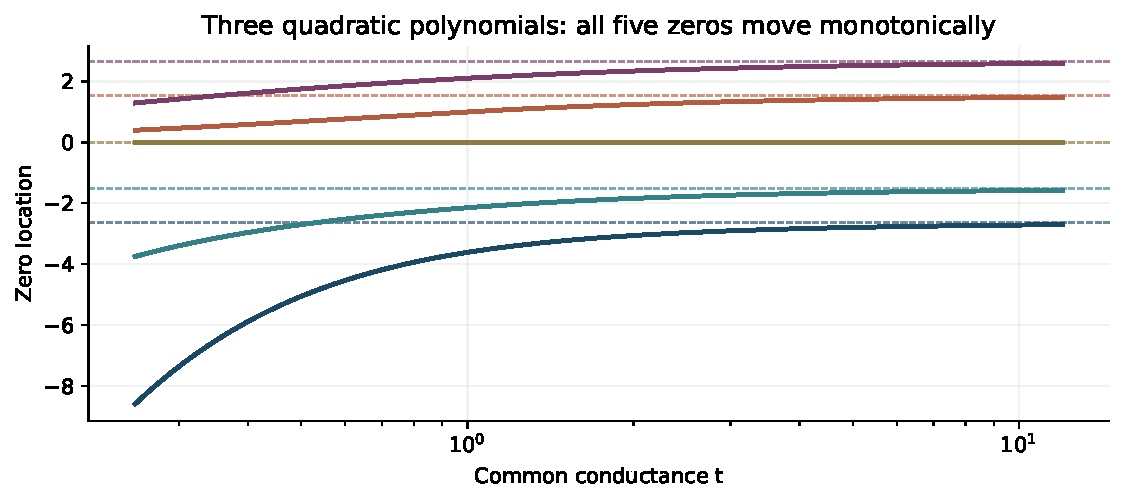
\includegraphics[width=.92\textwidth]{figures/quadratic_flow.pdf}
 \caption{The five graph zeros for three quadratic inputs.
 Dashed lines are the critical points of the input product.
 The zero at zero is fixed; all ordered curves are nondecreasing.
 The exact mean gap is $8/(15t)$.}
 \label{fig:quadratics}
\end{figure}

\subsection{A stronger collision used in verification}

The exact checker also uses $p_1=z^2$, $p_2=z(z-2)$, $p_3=(z-1)(z-3)$,
with path conductances $1$ and $4/3$.  It obtains
\[
 \mathcal P_G(z)=\tfrac43z^2(6z^3-16z^2-7z+26).
\]
At zero the input multiplicities are $2,1,0$.  The forced contribution
is $(2-1)+(1-1)=1$, while the one-dimensional complementary matrix
vanishes, adding one more zero.  Increasing the second conductance to
$5/3$ removes this extra nullity; the order at zero becomes one.  The
total movement of all ordered zeros is exactly $1/5$.

\section{Verification, reproducibility, and formalization}

\subsection{What was checked}

The human proof establishes the universal statements.  The computational
checks are independent finite checks of the normalization, signs,
repeated-root behavior, and edge-update formulas that are easy to get
wrong in this calculation.

The script \path{code/verify_graph.py} works with exact rational matrices
and polynomials in SymPy.  It forms the graph polynomial directly as
\[
 \det\bigl(L\diag(p_1,\ldots,p_n)+\diag(p_1',\ldots,p_n')\bigr)
\]
and compares it with the characteristic polynomial of the independently
constructed compressed matrix.  The check uses the ambient $N$-dimensional
matrix, which annihilates $\boldsymbol1_N$, and divides its characteristic
polynomial by the corresponding extra factor $z$.  This avoids choosing
an approximate orthonormal basis.

The recorded runs check six base examples: two one-vertex derivative
identities (including a constant output) as boundary checks, a two-vertex graph, a path with a tuned
shared-root collision, a triangle with mixed multiplicities, and a
four-cycle with common roots.  Four positive edge updates test both
strengthening an existing edge and inserting an absent one.  Each checks
the exact rank-one matrix identity, tree-weight normalization, and trace
displacement.  The collision formula is checked at every distinct input
root in each example.  All recorded checks passed.

The plots use numerical eigenvalues of symmetric matrices and are labelled
as illustrations.  Their underlying data and formulas are included.  They
are not interval-certified numerical computations of Dirichlet zeros.

\subsection{Reproduction}

From this directory, run:
\begin{verbatim}
python3 code/verify_graph.py
python3 code/illustrate.py
latexmk -pdf -interaction=nonstopmode -halt-on-error report.tex
\end{verbatim}
The first command writes exact JSON results to \path{checks/graph_checks.json};
its console output was recorded in \path{checks/graph_checks.txt}.
The second produces the plot PDFs, PNGs, and CSV data.
\path{requirements.txt} records the Python package versions used here.
The PDF was compiled with pdfLaTeX and rendered for visual inspection.

\subsection{A dependency plan for Lean}

The new theorems are not supplied as Lean-checked results.  A useful
formalization order would be the following.
\begin{enumerate}
 \item Define the graph derivative polynomial by the division-free
 principal-minor expansion.  Prove equality with the polynomial matrix
 determinant.  This separates algebra from graph combinatorics.
 \item Prove the bordered-determinant/compression identity for a real
 diagonal matrix and a block-incidence map $V$.  Define $L^+$ by its
 inverse on $\boldsymbol1^\perp$; no analytic generalized-inverse theory
 is necessary for this finite statement.
 \item Derive ordered eigenvalue monotonicity, the trace identity, and the
 rank-one update.  The transport formula can first be stated as the
 explicit sum of ordered displacements, avoiding any measure theory.
 \item Add the rooted-forest interpretation through the matrix-tree
 theorem.  The electrical resistance formula is then a finite identity
 in $L^+$ and the integer degree vector.
 \item For entire functions, formalize the locally uniform logarithmic
 derivative expansion and the strict imaginary-part inequality.  Prove
 the collision lemma for a Hermitian analytic matrix with negative
 definite derivative on its kernel.
 \item Instantiate the entire theorem with phase-real primitive
 Dirichlet completions, importing the upstream zero-location statement.
\end{enumerate}
This plan does not replace an executable proof file, and no unproved
placeholder is represented as a completed formalization.

\subsection{Remaining mathematical questions}

The finite transport law suggests two precise further problems.  First,
can one choose a canonical regularization of the displacement of
\emph{all} completed Dirichlet zeros and obtain an infinite analogue of
the resistance formula?  Second, which graph optimizes a chosen maximum
zero displacement subject to a conductance budget and prescribed input
degrees?  The first needs a genuine convergence argument; the second
leads to minimizing the largest eigenvalue of $B_G$.  Neither is needed
for the proved results above, and neither is claimed solved here.

\begin{thebibliography}{99}
\bibitem{grhsource}
L. Sernau (repository publisher), \emph{GRH for Dirichlet $L$-functions, in Lean 4},
revision \path{72fead102f663d5c7a407964a13dc0cf9d977207} (2026).
The compact README credits the proof to Levent Alp\"oge with Claude;
the repository presents a shorter rewriting of that proof.
README and \path{grh-compact/src/Statements.lean}, \path{src/Main.lean}.
\url{https://github.com/lsernau/grh-lean}.

\bibitem{grhguide}
Same repository, \path{grh-compact/GUIDE.md}, \path{src/New/Main.lean},
\path{src/New/Endgame/PrimeError.lean},
\path{src/New/Endgame/OneSidedCriterion.lean}, and
\path{src/Lib/Analytic/Landau/PolarLandau.lean}, at the same revision.
Exact paths and blob hashes are recorded in \path{provenance/source_manifest.json}.

\bibitem{proveit}
V. Reshetnikov, \emph{ProveIt}, \path{Analysis/GeneralizedRiemannHypothesis},
revision \path{4d7990202f9f106b2ffe8c209f073ad01d5e1987} (2026).
\url{https://github.com/VladimirReshetnikov/ProveIt/tree/main/Analysis/GeneralizedRiemannHypothesis}.
The inspected inventory includes 61 organized packets and 39 later incoming archives.

\bibitem{leanstatement}
Lean FRO and Mathlib Initiative, \emph{Lean verification of the Riemann
Hypothesis}, joint statement, 21 November 2026.
\url{https://leanprover-community.github.io/blog/posts/riemann-hypothesis/}.

\bibitem{wikipedia}
Wikipedia contributors, \emph{Riemann hypothesis}, retrieved 26 November 2026.
\url{https://en.wikipedia.org/wiki/Riemann_hypothesis}.
Used as the requested contextual source, not as the proof of the new results.

\bibitem{forests}
P. Chebotarev and E. Shamis, \emph{Matrix-Forest Theorems},
manuscript (1994--1997), revised preprint (2023).
\url{https://arxiv.org/abs/math/0602575}.

\bibitem{pereira}
R. Pereira, \emph{Differentiators and the geometry of polynomials},
Journal of Mathematical Analysis and Applications \textbf{285} (2003), 336--348.
\url{https://doi.org/10.1016/S0022-247X(03)00465-7}.

\bibitem{bb}
J. Borcea and P. Br\"and\'en, \emph{The Lee--Yang and P\'olya--Schur
programs. I. Linear operators preserving stability},
Inventiones Mathematicae \textbf{177} (2009), 541--569.
\url{https://arxiv.org/abs/0809.0401}.

\bibitem{reiffenstein}
J. Reiffenstein, \emph{Higher-order interlacing for matrix-valued meromorphic
Herglotz functions}, Journal of Mathematical Analysis and Applications
\textbf{514} (2022), 126260.
\url{https://arxiv.org/abs/2108.10746}.

\bibitem{simonov}
S. Simonov and H. Woracek, \emph{Local spectral multiplicity of selfadjoint
couplings with general interface conditions}, Integral Equations and
Operator Theory \textbf{96} (2024), article 18.
\url{https://doi.org/10.1007/s00020-024-02767-6}.

\bibitem{dlmfdirichlet}
NIST Digital Library of Mathematical Functions, \S25.15,
\emph{Dirichlet $L$-functions}, definitions and functional equations.
\url{https://dlmf.nist.gov/25.15}.

\bibitem{dlmfzeta}
NIST Digital Library of Mathematical Functions, \S25.4,
\emph{Reflection formulas}, including Riemann's completed $\xi$-function.
\url{https://dlmf.nist.gov/25.4}.
\end{thebibliography}

\end{document}
